% ============================ Enrico Ribiani 16-03-2021 ====================================================================
% Base per i documenti  
\documentclass[12pt]{article}
% ------------ pacchetti necessari ----------------
\usepackage[a4paper, total={6in, 8in},margin=1in]{geometry} % formattazione decente della pagina
\usepackage{graphicx}                            % need for figure
\usepackage{amsmath}
\usepackage{amsfonts}                            % if you want the fonts
\usepackage{amssymb}                             % if you want extra symbols
\usepackage{graphicx}  
\renewcommand{\figurename}{Figura}  
\renewcommand{\contentsname}{Indice}                        % need for figures
\usepackage{mathptmx}
\usepackage{float}                               % serve per mettere tabelle e immagini dove si vuole 
\usepackage[utf8]{inputenc}
\usepackage{textcomp}
\usepackage[hang,flushmargin,bottom]{footmisc}   % footnote format
\usepackage{fancyhdr, lastpage}
\usepackage{titlesec}
\usepackage[table,dvipsnames]{xcolor}
%\pagestyle{fancy}
%\renewcommand{\headrulewidth}{0pt}
%\renewcommand*\contentsname{Indice}
\titleformat{\section}{\normalsize\bfseries}{\thesection.}{1em}{}	% required for heading numbering style
\titleformat*{\section}{\Large\bfseries}
\titleformat*{\subsection}{\large\bfseries}
%\usepackage{siunitx}
%\usepackage{tikz}
\usepackage{circuitikz}
\usepackage{multicol}
%\usepackage[siunitx]{circuitikz}
\usepackage{multirow}
\usepackage{tikz}
\usepackage{amsmath}
\usetikzlibrary{angles,quotes}
\usepackage{placeins}

\usepackage{wasysym}
%===================links=================
\usepackage{hyperref}
\hypersetup{
    colorlinks=true,
    linkcolor=darkgray,
    filecolor=Green,      
    urlcolor=Cyan,
    pdftitle={SAMPLE},
    pdfpagemode=FullScreen,
    }
%===================inizio pagina del titolo=================
\begin{document}
\begin{titlepage}
	\begin{center}
		% ------------------ inizio immagine logo ----------
		\begin{figure}
			\centering
			
\includegraphics[scale=1.3]{/home/r1bbi/Documenti/latec/logo.png}

		\end{figure}
		% ------------------ fine immagine logo ----------
		% ------------------ fine immagine logo ----------
		-------------------------------------------------------------------------------------\\
		\vspace{2\baselineskip}
		\large Prova n°6
		\hfill
		\large $5^a$   AUB\\
		\begin{flushleft}
			\large Enrico Ribiani\\
			\large Daniel Graziadei\\
			\large Gruppo 11\\
		\end{flushleft}


		\vfill

		\Huge{\textbf{Raddrizzatore controllato monofase a semionda}}\\
		\vfill
		\vfill
		\large{16-3-2023}
	\end{center}
	%=============== fine pagina titolo ===============
\end{titlepage}
\thispagestyle{empty}
\tableofcontents
\newpage
\setcounter{page}{1}
\vskip 1cm
\section{Raddrizzatore attivo}
\subsection{Scopo}
Verificare il comportamento qualitativo in modo sperimentale delle tensioni e correnti in in-
gresso e sul carico di un raddrizzatore attivo simulato con MultiSim.\\

\subsection{Schema}
\begin{figure}[!h]
	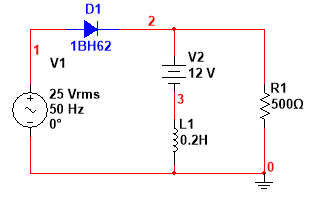
\includegraphics[scale=0.7]{schema-es1.PNG}
\end{figure}

\subsection{Materiale e Strumenti}
\begin{multicols}{2}
	\begin{itemize}
		\item Generatore AC 25V
		\item Generatore DC 12V
		\item diodo 1BH62
		\item Resistenza da $500\Omega$
		\item Induttore 0.2H
	\end{itemize}
	\vfill\null
	\columnbreak
	\begin{itemize}
		\item Oscilloscopio
	\end{itemize}
	\vfill\null
\end{multicols}

\subsection{Contenuti Teorici}
Questo circuito ha una funzione molto importante poichè il generatore in continua rappresenta la forza controelettromotrice
generata dall'avvolgimento di un motore che in determinate condizioni ha valore costante.\\
Il generatore avrà la funzione di far condurre la corrente al diodo solo quando la tensione ai suoi capi
supererà la V2.\\
Inoltre avendo un carico di tipo induttivo la corrente sarà sfasata e la tensione presenterà un picco negativo
come visto nell'esperienza precedente.\\
\subsection{Raccolta dati}
\begin{figure}[H]
	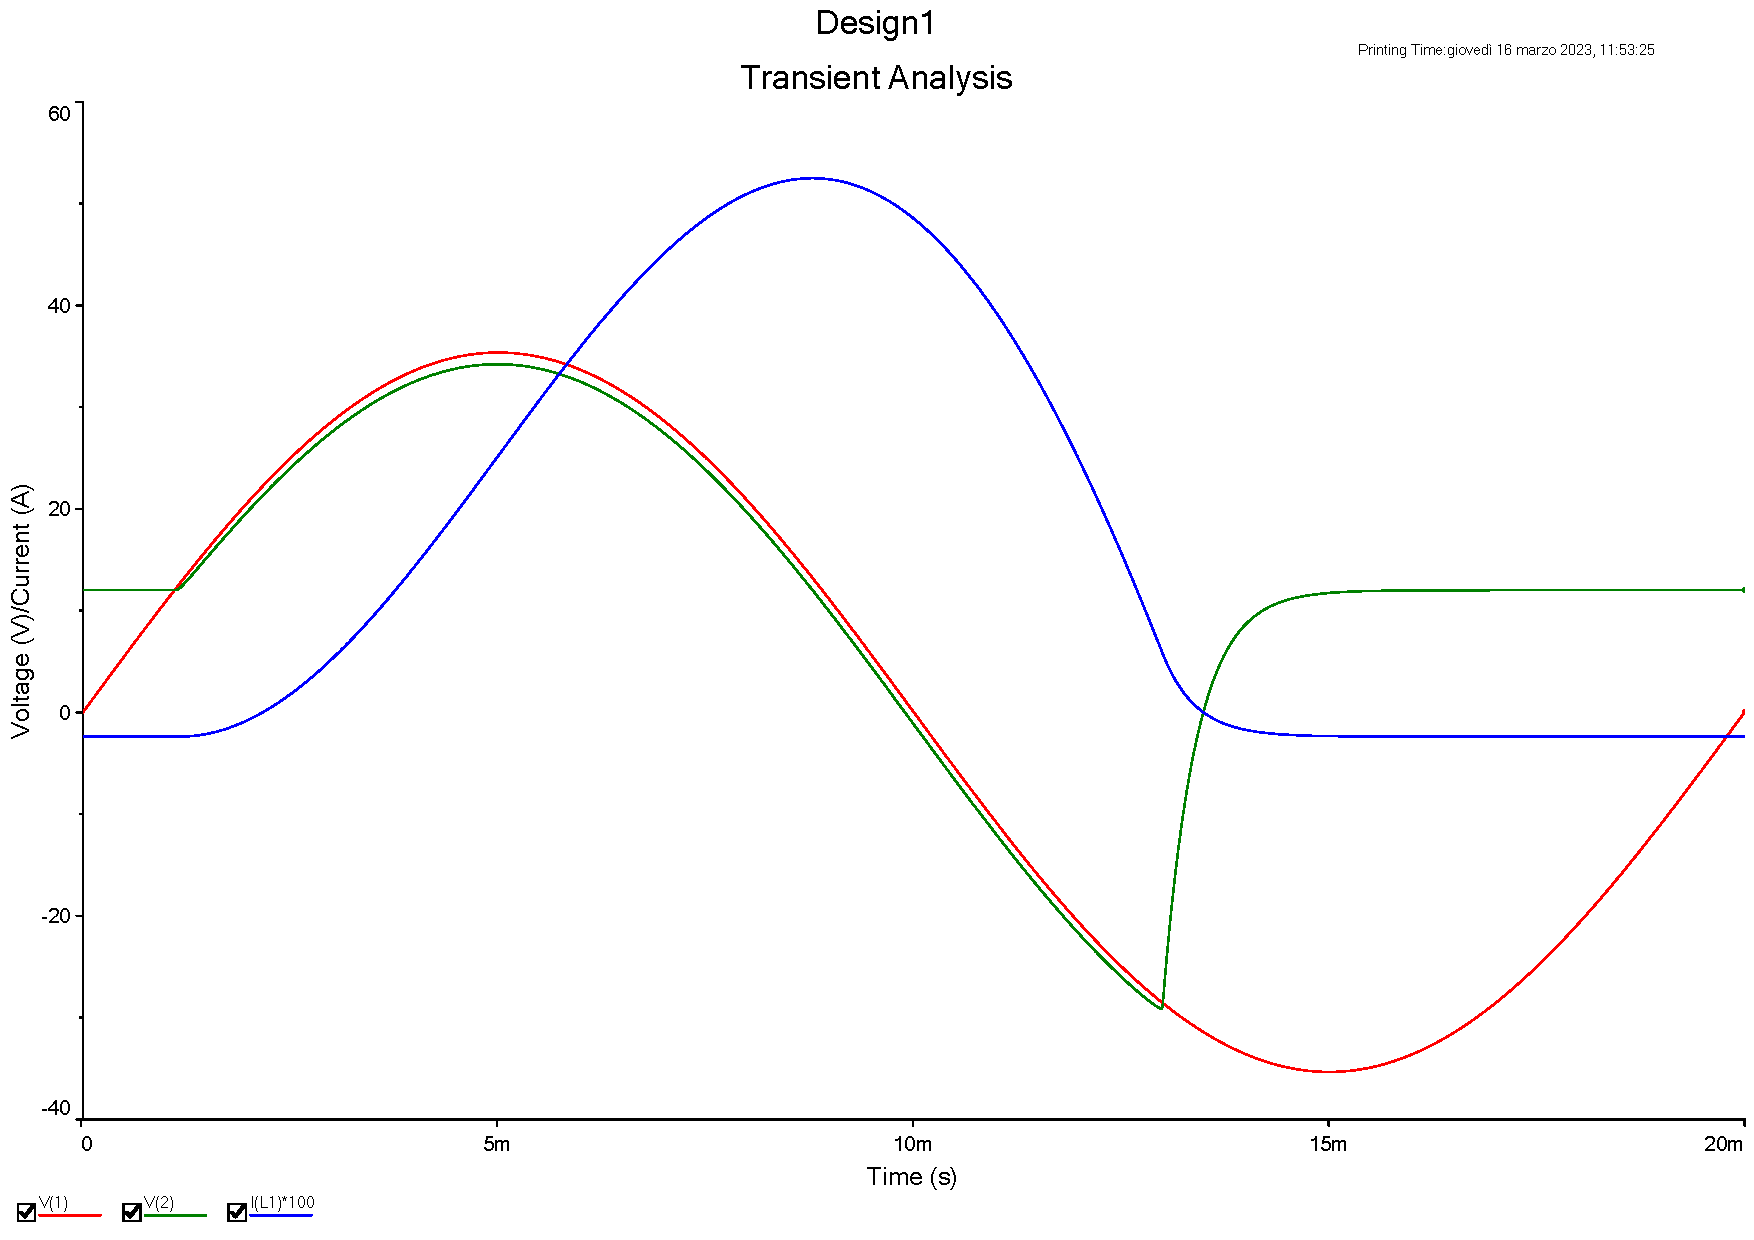
\includegraphics[scale=0.5]{osc-es1.pdf}
\end{figure}
\subsection{Analisi critica dei risultati e conclusioni}
Osservando il grafico ricavato dal software di simulazione MultiSim possiamo notare come la corrente (in blu)
inizi a crescere contemporaneamente alla tensione sul diodo (in verde) poichè la tensione ai suoi capi
ha superato quella del generatore.\\
Possiamo notare anche il picco di tensione negativa e lo sfasamento della corrente dovuto alla smagnetizzazione
dell'induttore.\\
Lo scopo quindi è verificato perchè il comportamento sperimentale segue esattamente la previsione teorica.\\
\newpage
\section{Controllo di fase}
\subsection{Scopo}
Osservare il comportamento di un raddrizzatore monofase a frequenza di rete con controllo di fase a frequenza
di rete [\textit{f=50Hz}].\\
E verificare che il comportamento rispetti le previsioni teoriche con vari angoli di fase.\\
\subsection{Schema}
\begin{figure}[H]
	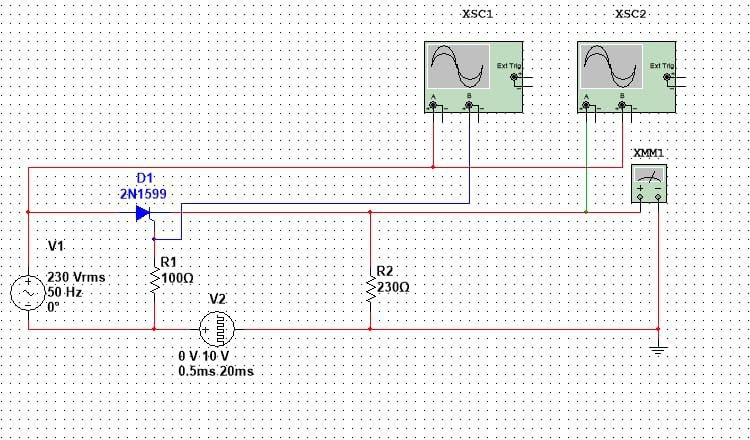
\includegraphics[scale=0.4]{schema.jpg}
\end{figure}
\subsection{Materiale e Strumenti}
\begin{multicols}{2}
	\begin{itemize}
		\item Generatore AC 230V
		\item Generatore di impulsi 50HZ
		\item Tiristore SCR
		\item Resistore da $100\Omega$
		\item Resistore da $230\Omega$
	\end{itemize}
	\vfill\null
	\columnbreak
	\begin{itemize}
		\item Oscilloscopio
		\item Voltmetro
	\end{itemize}
	\vfill\null
\end{multicols}
\subsection{Contenuti Teorici}
Il circuito si controlla attraverso il gate del tiristore su cui arrivano gli impulsi del generatore.\\
Variando l'angolo di inneso possiamo modulare il valore della tensione.\\
Durante la prima semionda positiva, il tiristore si comporta come un circuito aperto fino all'impulso di
commutazione OFF-ON sul gate.\\ Da qui la Vu sarà uguale alla Vi e sul carico si localizzerà la Vi fino al
valore impostato di angolo di fase d'innesco del tiristore.\\
Con la semionda negativa, la corrente si annulla e determina lo spegnimento del tiristore che rimane in
stato d'interdizione.\\
(Vu=0) Durante la successiva semionda positiva l'SCR è in grado di condurre ma lo fa dopo il segnale
d'impulso sul gate.\\
Quindi aumentanto l'angolo di innesco la tensione in uscita diminuirà.\\
Il circuito verrà testato con angolo di innesco da 0° a 180° aumentando di 30° alla volta.\\
\subsection{Raccolta dati}
\begin{center}
\begin{figure}[H]
   \caption{ancolo di innesco a 0 gradi}
   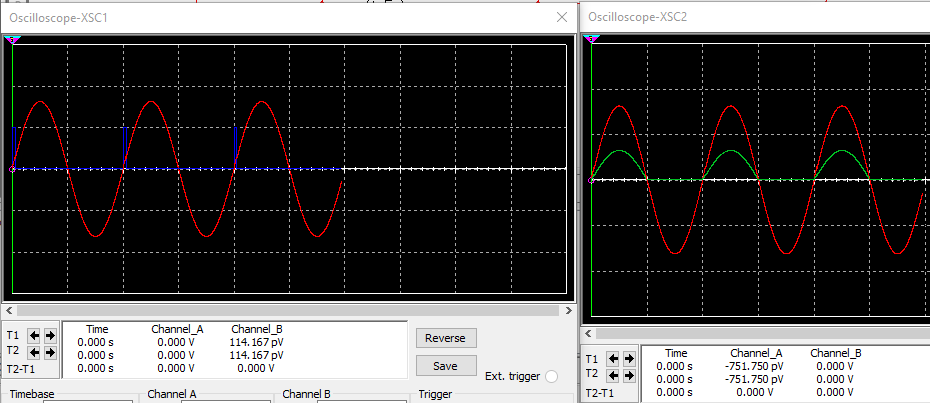
\includegraphics[scale=0.7]{Grafico 0.PNG}
\end{figure}


\begin{figure}[H]
\caption{ancolo di innesco a 30 gradi}
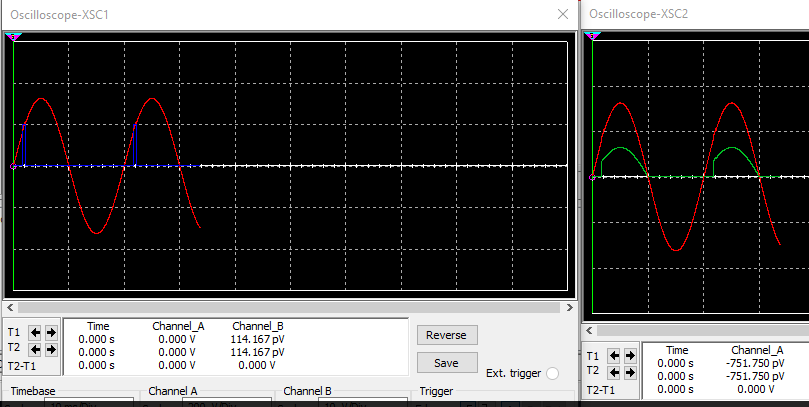
\includegraphics[scale=0.7]{Grafico 30.PNG}
\end{figure}


\begin{figure}[H]
\caption{ancolo di innesco a 60 gradi}
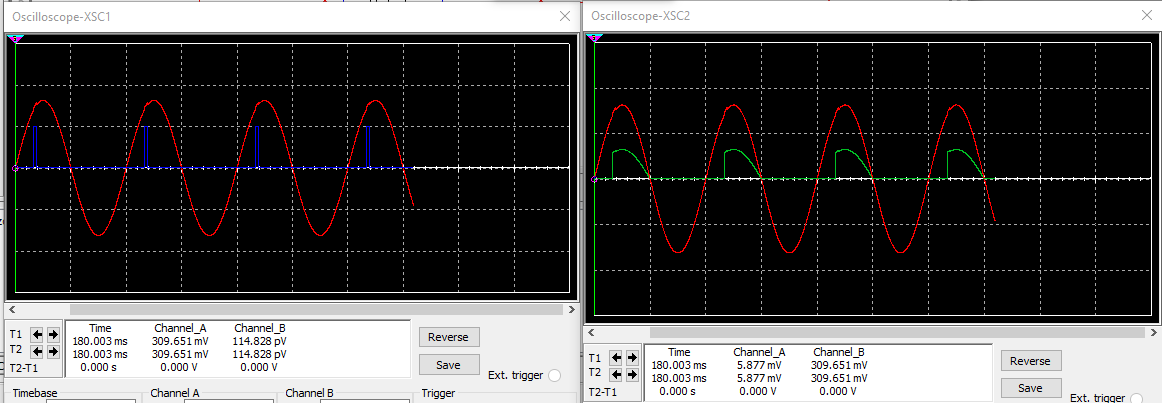
\includegraphics[scale=0.7]{Grafico 60.PNG}
\end{figure}

\begin{figure}[H]
    \caption{ancolo di innesco a 120 gradi}
    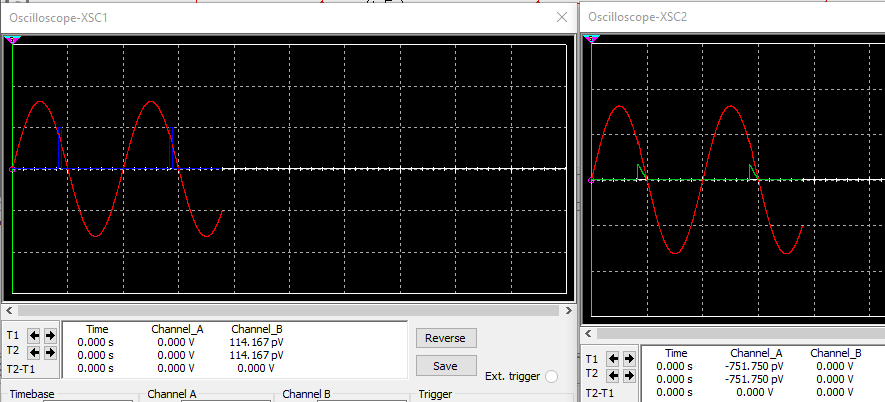
\includegraphics[scale=0.7]{Grafico 120.PNG}
\end{figure}


\begin{figure}[H]
    \caption{ancolo di innesco a 150 gradi}
    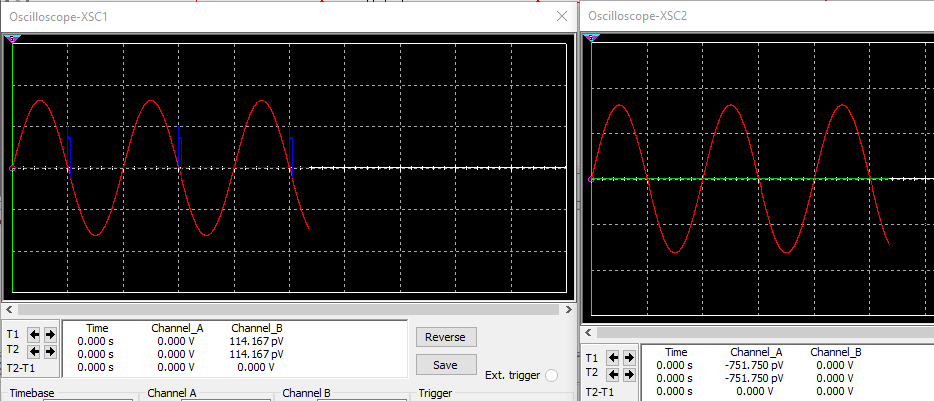
\includegraphics[scale=0.7]{Grafico 150.PNG}
\end{figure}

\begin{figure}[H]
    \caption{ancolo di innesco a 180 gradi}
    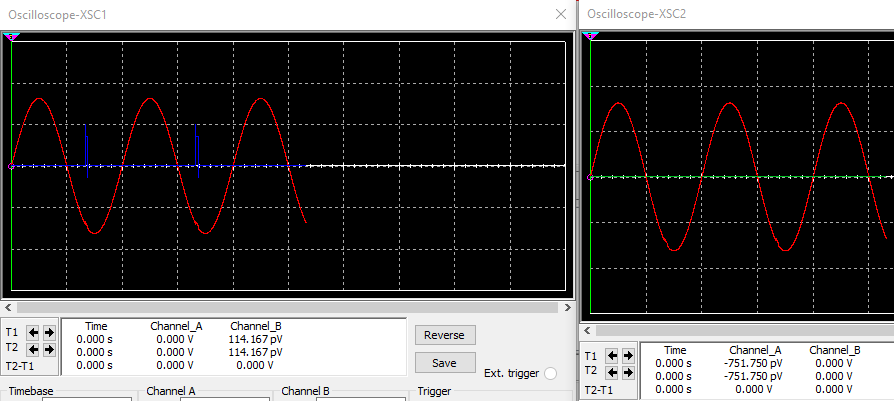
\includegraphics[scale=0.7]{Grafico 180.PNG}
\end{figure}

\end{center}
\newpage
\subsection{Calcoli}

Sappiamo che t30" (delay per ottenere un angolo di innesco di 30°) è uguale a 1,67ms  e ovviamente
conosciamo l'angolo di innesco desiderato, non ci resta che calcolare il tempo con la formula ricavata
dalla proporzione xt:x°=t30":30°.\\
$xt=\frac{X°\cdot t30"}{30°} [s]$
\subsection{Analisi critica dei risultati e conclusioni}
Nei grafici possiamo vedere l'impulso di innesco rappresentato nel grafico a sinistra, sovrapposto alla tensione 
di ingresso, in rosso.\\
Sul grafico a sinistra invece possiamo osservare la tensione di uscita, in verde, si può notare come il 
comportamento di quest'ultima cambi a seconda dell'angolo di innesco.\\
Infatti la tensione d'uscita con angolo di innesco nullo è massima mentre è minima a 120 gradi e nulla a partire
dai 150 gradi.\\
Possiamo affermare che il circuito si è comportato esattamente come avevamo previsto, infatti il tensione efficace
della tensione aumenta in modo inversamente proporzionale all'angolo di innesco.\\
\end{document}


